\documentclass[12pt,a4paper]{article}
\usepackage{classeRapport} % template INSA
\usepackage{hyperref} % lien tableofcontents + url
\usepackage{graphicx} % pour les images
\usepackage{listings} % pour mettre du code
\usepackage{color} % pour la couleur dans le code
\usepackage{amsmath} % pour les matrices
\usepackage{float} % pour le [H] des figures

\hypersetup{ % couleur des liens
    colorlinks=true,
    linkcolor=black,
    filecolor=black,      
    urlcolor=blue,
}

\definecolor{backcolour}{rgb}{0.95,0.95,0.92}
 
%%%%
\definecolor{mygreen}{RGB}{28,172,0} % color values Red, Green, Blue
\definecolor{mylilas}{RGB}{170,55,241}

\lstdefinestyle{mystyle}{
    backgroundcolor=\color{backcolour},   
    basicstyle=\footnotesize,
    breakatwhitespace=false,         
    breaklines=true,                 
    captionpos=b,                    
    keepspaces=true,                 
    numbers=left,                    
    showspaces=false,                
    showstringspaces=false,
    showtabs=false,                  
    tabsize=2,
    %%%%
    language=Matlab,
    morekeywords={matlab2tikz},
    keywordstyle=\color{blue},
    morekeywords=[2]{1}, keywordstyle=[2]{\color{black}},
    identifierstyle=\color{black},
    stringstyle=\color{mylilas},
    commentstyle=\color{mygreen},
    showstringspaces=false, % without this there will be a symbol in the places where there is a space
    numberstyle={\tiny \color{black}}, % size of the numbers
    numbersep=9pt, % this defines how far the numbers are from the text
    emph=[1]{for,end,break},emphstyle=[1]\color{red}, % some words to emphasise
}

\lstset{style=mystyle}

\begin{document}

\PageDeGarde
{Images/TemplateINSA/rien} % image sur la page de garde
{Filtre de Kalman/Suivi d'objets} % titre principal
{Mini-projet TSA} % sous-titre
{Mehdi \textsc{ABOUZAID}\\
 Damien \textsc{TOOMEY}\\
 --\\
 À l'attention de \\ M. \textsc{HÉRAULT}} % nom
{TSA - ASI - 2017-2018} % bas de page

\Page{INSALogo}{rien.png} % logo de bas de page (en bas a droite)

\newpage
\tableofcontents

\newpage
\section{Étude bibliographique sur le modèle}
\subsection{Présentation} 

\indent Le filtre de Kalman est un filtre à réponse impulsionnelle infinie (RII), c’est-à-dire qu'il est basé uniquement sur les valeurs en entrée du filtre ainsi que sur les valeurs antérieures de cette même réponse. Sa fonction est donc d'estimer les états d’un système dynamique à partir d'une série de mesures incomplètes ou bruitées.

Le filtre de Kalman fait appel à la dynamique de la cible qui définit son évolution dans le temps pour obtenir de meilleures données, éliminant ainsi l'effet du bruit. Ces données peuvent être calculées pour faire du filtrage ou pour de la prédiction.

\subsection{Origine}

\indent Le filtre de Kalman a été nommé ainsi, suite à sa conception dans les années 1950 par Rudolf Kalman, mathématicien et automaticien américain d'origine hongroise. Pourtant, dès le XIX\textsuperscript{ème} siècle, Thorvald Nicolai Thiele, astronome danois, puis au XX\textsuperscript{ème} siècle, Peter Swerling, automaticien américain, avaient déjà tous les deux développé un algorithme similaire au filtre de Kalman.

\indent Stanley Schmidt est reconnu comme ayant réalisé la première mise en œuvre du filtre. C'était lors d'une visite de Rudolf Kalman à la NASA Ames Research Center qu'il vit le potentiel de son filtre pour l'estimation de la trajectoire pour le programme Apollo. Ceci a conduit à l'utilisation du filtre dans l'ordinateur de navigation.

\subsection{Fonctionnement}

\indent L'algorithme fonctionne en deux étapes, une étape de prédiction et une étape de mise à jour. La phase de prédiction utilise l'état estimé de l'instant précédent pour produire une estimation de l'état courant. Une fois les observations de l’instant courant obtenues, la seconde phase de mise à jour consiste à apporter une correction de l'état prédit dans le but d'obtenir une estimation plus précise. L'algorithme du filtre de Kalman est un processus dit récursif et markovien. Cela signifie que pour estimer l'état courant, seules l'estimation de l'état précédent et les mesures actuelles sont nécessaires, aucune autre information supplémentaire n’est requise. \\

Le filtre de Kalman est limité aux systèmes linéaires. Cependant, la plupart des systèmes physiques sont non linéaires. Le filtre n'est donc optimal que sur une petite plage linéaire des phénomènes réels. Une grande variété de filtres de Kalman a été depuis développée à partir de la formulation originale dite filtre de Kalman simple. Par exemple, Schmidt a développé le filtre de Kalman étendu, applicable aux phénomènes non linéaires. 

\paragraph{Modèles du filtre}
~~\\
\begin{itemize}
	\item[] Modèle de dynamique ou système : \\
$x_k=Ax_{k-1}+q$ \\
$x_k|x_{k-1} \sim  \mathcal{N}(x_k|Ax_{k-1},\,Q)\,$
	\item[] 
	\item[] Modèle d'observation : \\
$y_k=Hx_k+r$ \\
$y_k|x_k \sim  \mathcal{N}(y_k|Hx_k,\,R)\,$
\end{itemize}

\paragraph{Distributions des états et des observations}
~~\\
\begin{itemize}
	\item[] Pour les états : \\
	$P(x_k|y_{1:k-1}) \sim \mathcal{N}(x_k|m_k^-,\,P_k^-)\,$ \\
	$P(x_k|y_{1:k-1}) \sim \mathcal{N}(x_k|m_k^-,\,P_k^-)\,$
	\item[]
	\item[] Pour les observations : \\ 
	$P(x_k|y_{1:k-1}) \sim \mathcal{N}(x_k|m_k^-,\,P_k^-)\,$
\end{itemize}

\paragraph{Prédiction}
~~\\
\begin{itemize}
	\item[] Connaissant x[0:k-1] et y[1:k-1], on cherche à estimer x[k] : \\
	$P(x_k|y_{1:k-1}) \sim \mathcal{N}(x_k|m_k^-,\,P_k^-)\,$
	\item[] On applique le modèle de dynamique : \\
	$m_k^- = Am_{k-1}$ \\
	$P_k^- = AP_{k-1}A^T+Q$ 
\end{itemize}

\paragraph{Mise à jour} 
~~\\
\begin{itemize}
	\item[] Connaissant x[0:k-1] et y[1:k], on cherche à estimer x[k]: \\
	$P(x_k|y_{1:k}) \sim \mathcal{N}(x_k|m_k,\,P_k)\,$
	\item[] On corrige la prédiction de l'étape précédente par l'observation $k$ : \\
	$v_k=y_k-Hm_k^-$ \\
	$S_k = HP_k^-H^T+R$ \\
	$K_k = P_k^-H^TS_k^{-1}$ \\
	$m_k=m_k^-+K_kv_k$ \\
	$P_k=P_k^- - K_kS_kK_k^T$ \\
\end{itemize}

\paragraph{Détail des matrices et vecteurs}
~~\\
Nous choisissons le modèle de l'accélération constante au vu des données que avons choisies. \\

Matrice de dynamique/transfert/système
\[ A=\begin{pmatrix}
	1 & 0 & dt & 0 & 0 & 0 \\
	0 & 1 & 0 & dt & 0 & 0 \\
	0 & 0 & 1 & 0 & dt & 0 \\
	0 & 0 & 0 & 1 & 0 & dt \\
	0 & 0 & 0 & 0 & 1 & 0 \\
	0 & 0 & 0 & 0 & 0 & 1 \\
\end{pmatrix} \] 

Matrice d'observation
\[ H= \begin{pmatrix}
	1 & 0 & 0 & 0 & 0 & 0 \\
	0 & 1 & 0 & 0 & 0 & 0 \\
\end{pmatrix} \]

Vecteur d'état
\[m_k=\begin{pmatrix}
	x \\
	y \\
	\dot{x} \\
	\dot{y} \\
	\ddot{x} \\
	\ddot{y}
\end{pmatrix}\] 

Bruit de transition
\[ Q= \begin{pmatrix}
	a & 0 & 0 & 0 & 0 & 0 \\
	0 & b & 0 & 0 & 0 & 0 \\
	0 & 0 & c & 0 & 0 & 0 \\
	0 & 0 & 0 & d & 0 & 0 \\
	0 & 0 & 0 & 0 & e & 0 \\
	0 & 0 & 0 & 0 & 0 & f \\
\end{pmatrix} \quad \forall a,b,c,d,e,f \in {\rm I\!R} \]


Bruit d'observation
\[ R=\begin{pmatrix}
	g & 0 \\
	0 & h \\
\end{pmatrix} \quad \forall g,h \in {\rm I\!R} \]

Covariance de l'état initial
\[ p_0= \begin{pmatrix}
	i & 0 & 0 & 0 & 0 & 0 \\
	0 & j & 0 & 0 & 0 & 0 \\
	0 & 0 & k & 0 & 0 & 0 \\
	0 & 0 & 0 & l & 0 & 0 \\
	0 & 0 & 0 & 0 & m & 0 \\
	0 & 0 & 0 & 0 & 0 & n \\
\end{pmatrix} \quad \forall i,j,k,l,m,n \in {\rm I\!R} \]




\newpage
\section{Étude bibliographique sur l'application}
\paragraph{}
	
	Le suivi d'objet correspond au fait de localiser un objet dans une vidéo ou une séquence d'images. \\
	
	Dans les années 1960, le filtre de Kalman a été utilisé pour la première fois lors de la mission Apollo pour estimer la trajectoire de la fusée allant sur la Lune. Ce filtre est aussi utilisé pour corriger la trajectoire de missiles et calculer l'altitude d'une fusée.

	A partir des années 1990, le filtre de Kalman s'est propagé à la société civile avec les GPS\footnote{GPS : Global Positioning System} (système de positionnement global). \\

	Le filtre de Kalman permet également la fusion de données pour avoir une meilleur estimation de chaque donnée. Par exemple, si une voiture est équipée de trois capteurs :
\begin{itemize}
\item[•] système de mesure inertiel (IMU\footnote{IMU : Inertial Measurement Unit}) : mesure l'accélération et la vitesse angulaire de la voiture 
\item[•] Odomètre : donne la position relative de la voiture 
\item[•] GPS : donne la position absolue de la voiture,
\end{itemize}	 
le filtre de Kalman permet de prendre en compte les données de chaque capteur et estimer une position plus précise de la voiture. \\

	Aujourd'hui, il est possible de suivre un ou plusieurs objets dans une vidéo, en temps réel ou non, la position de la caméra étant fixe ou non. Le suivi d'objets est entre autres utilisé dans le domaine de sécurité, la réalité augmentée et le contrôle de la circulation. Si l'objet est détecté, sa position est corrigée sinon elle est prédite. \\

	Dans le cadre de notre étude, nous nous concentrerons uniquement sur le suivi d'objets (tracking). \\
\indent Vu le délai très court qui nous est imparti, nous n'étudierons le suivi d'un unique objet avec une caméra stationnaire (arrière plan constant).

\newpage
\section{Présentation du jeu de données choisi ou construit}
\subsection{Vidéo 1 : \emph{singleball.mp4}}

Pour notre projet, nous avons utilisé une vidéo nommée \emph{singleball.mp4} trouvée dans les exemples fournis par \emph{Matlab}. La vidéo correspond à une balle verte qui roule sur un sol foncé. Au cours de la vidéo, la balle passe sous une boîte en carton pendant un court instant puis réapparaît de l'autre de celle-ci. Pour faciliter le suivi de l'objet, la caméra est stationnaire (l'arrière-plan ne change pas). \\

Informations concernant la vidéo \emph{singleball.mp4} :
\begin{itemize}
\item[] durée : $ 1.5 \; s $
\item[]	largeur : 480
\item[] hauteur : 360
\item[]	nombre d'images par seconde : 30
\item[] bits par pixel : 24
\item[] format : RGB24
\end{itemize}

\subsection{Vidéo 2 : \emph{singleballhomemade.mp4}}

Nous souhaitions tester le code avec une seconde vidéo. Nous avons donc réalisé une vidéo avec la même mise en scène (caméra stationnaire), à savoir une balle qui suit une trajectoire et qui est cachée par un obstacle (un portefeuille dans notre cas) pendant un court instant puis réapparaît de l'autre côté de l'obstacle.  \\

Informations concernant la vidéo \emph{singleballhomemade.mp4} :
\begin{itemize}
\item[] durée : $ 3.0420 \ s $
\item[]	largeur : 1280
\item[] hauteur : 720
\item[]	nombre d'images par seconde : 30
\item[] bits par pixel : 24
\item[] format : RGB24 \\
\end{itemize}

\paragraph{}
Dans les deux vidéos, nous avons donc deux missions :
	\begin{itemize}
		\item[•] corriger la position de la balle quand la balle est détectée
		\item[•] prédire la position de la balle quand elle passe sous la boîte (balle non détectée) \\
	\end{itemize}
	
Nous avons commencé par étudier la vidéo \emph{singleball.mp4}. Le code était donc bien adapté pour cette vidéo. En revanche, lorsque nous avons voulu tester le code avec la vidéo \emph{singleballhomemade.mp4}, nous avons remarqué que le code n'était pas générique et ne fonctionnait donc pas pour cette seconde vidéo. En fait, le traitement d'image ne détectait pas la balle alors qu'elle était visible. \\

Malheureusement, nous n'avons pas eu le temps d'améliorer le code pour qu'il soit adapté à l'autre vidéo.

\newpage
\section{Explication de l'implémentation}
\paragraph{}

	Nous avons trouvé un code\footnote{Code accessible dans /Code/kalmanFilterForTracking.m} \emph{Matlab} sur le site \href{https://fr.mathworks.com/help/vision/examples/using-kalman-filter-for-object-tracking.html}{MathWorks} qui applique un filtre de Kalman sur la vidéo \emph{singleball.mp4} mais cet exemple utilise la \emph{toolbox vision} qui n'est pas accessible sur la version académique de \emph{Matlab} de l'\emph{INSA}. \\
\indent Nous avons donc décidé de reproduire le code que nous avons trouvé sur ce site pour qu'il fonctionne sur la version académique. Nous avons obtenu le code suivant par nous-même et avec du code trouvé sur internet.
	
	Dans ce code, nous avons considéré que la vidéo pouvait contenir l'objet dès la première image, ainsi, nous supposons que nous n'avons pas d'image de la vidéo avec uniquement l'arrière plan. \\
	
	Le main se nomme \emph{ProjetTSA.m}. Le code est commenté, ce qui sert également d'explication. \\

\hrule
\phantom{}
\phantom{}

	Initialisation/Ré-initialisation du fichier.
	
\lstset{caption=ProjetTSA.m}
\lstinputlisting[firstnumber=1,firstline=1,lastline=4]{../Code/ProjetTSA.m}

\hrule
\phantom{}
\phantom{}

	Utilisation de l'entrée standard sur \emph{Matlab} pour permettre à l'utilisateur de choisir la vidéo qu'il souhaite étudier. Cela permet au programme de trouver le chemin vers le répertoire contenant la succession d'images.
	
\lstset{caption=ProjetTSA.m}
\lstinputlisting[firstnumber=6,firstline=6,lastline=29]{../Code/ProjetTSA.m}

\hrule
\phantom{}
\phantom{}
	
Tout d'abord, nous souhaitons ouvrir la vidéo dans \emph{Matlab}.

\lstset{caption=ProjetTSA.m}
\lstinputlisting[firstnumber=31,firstline=31,lastline=43]{../Code/ProjetTSA.m}

\hrule
\phantom{}
\phantom{}

Malheureusement, sur la version \emph{Matlab} 2017 de \emph{Linux} de l'INSA, la lecture de vidéo n'est pas possible. Nous avons donc sauvegardé chaque image de la vidéo en format \emph{png} et nous avons travaillé sur ces images.

\lstset{caption=ProjetTSA.m}
\lstinputlisting[firstnumber=45,firstline=45,lastline=53]{../Code/ProjetTSA.m}

\hrule

\subsection{Traitement d'image}

	Pour détecter l'objet, on compare deux images à la fois (l'image courante et l'image suivante). Par conséquent, l'utilisation de la fonction \emph{imabsdiff} peut entraîner l'apparition de deux objets car si l'image à l'instant $ k $ contient l'objet et l'image à l'instant $ k+1 $ contient également l'objet, la valeur absolue de la différence de ces deux images va faire apparaître deux objets. En fait, c'est le même objet à deux instants différents. Ainsi, quand on obtient le centre de masse avec \emph{regionprops}, il peut y avoir un ou deux centres de masse.
	
\lstset{caption=ProjetTSA.m}
\lstinputlisting[firstnumber=55,firstline=55,lastline=96]{../Code/ProjetTSA.m}

\hrule
\phantom{}
\phantom{}

	Comme la détection de l'objet est imprécise, la détection du centre de masse l'est aussi. En comparant l'image 1 et l'image 2 (comparaison A) puis l'image 2 et l'image 3 (comparaison B), la détection du centre de masse de l'objet de l'image 2 dans les comparaisons A et B ne sont pas les mêmes (mais proches). Pourtant nous savons qu'il s'agit du même objet au même instant. Le code suivant permet de faire la moyenne des centres de masse lorsqu'il s'agit du même objet au même instant :

\lstset{caption=ProjetTSA.m}
\lstinputlisting[firstnumber=98,firstline=98,lastline=156]{../Code/ProjetTSA.m}

\hrule
\phantom{}
\phantom{}

	On retire les positions \textbf{[ ]} en fin de vidéo car on considère qu'on n'aura pas à prédire ces positions (on considère que l'objet est hors champ de la caméra même si cela n'est pas nécessairement vrai) :

\lstset{caption=ProjetTSA.m}
\lstinputlisting[firstnumber=158,firstline=158,lastline=168]{../Code/ProjetTSA.m}

\hrule
\phantom{}
\phantom{}

	En raison d'imprécisions dans l'analyse d'image, il reste des points très proches mais il s'agit en fait des mêmes points donc nous faisons la moyenne de ces points. Nous avons décidé que si la distance entre deux points est inférieure à $ 3 $ alors il s'agit du même point ($<=3$ choisi de manière empirique).

\lstset{caption=ProjetTSA.m}
\lstinputlisting[firstnumber=170,firstline=170,lastline=181]{../Code/ProjetTSA.m}

\hrule
\phantom{}
\phantom{}

	Affichage des points détectés sur l'image binaire et sur l'image de départ en noir et blanc.

\lstset{caption=ProjetTSA.m}
\lstinputlisting[firstnumber=183,firstline=183,lastline=213]{../Code/ProjetTSA.m}

\hrule

\subsection{Filtre de Kalman}

	Appel de la fonction \emph{trackingObjet} pour appliquer le filtre de Kalman sur chaque positions de \emph{cell\_pos\_bis}.

\lstset{caption=ProjetTSA.m}
\lstinputlisting[firstnumber=215,firstline=215,lastline=223]{../Code/ProjetTSA.m}

\hrule
\phantom{}
\phantom{}

	Pour tester le filtre de Kalman avec ajustements de la vitesse, de l'accélération et $ dt = \; 1/30 \; s $ il faut dé-commenter les lignes 11 et 15 puis commenter les lignes 10 et 14 dans \emph{trackingObjet.m}. Les lignes 10 et 14 permettent d'appliquer le filtre de Kalman sans ajustement de la vitesse et de l'accélération avec $ dt $ choisi à la ligne 16 ou 21 dans \emph{ProjetTSA.m} selon la vidéo choisie.
\lstset{caption=trackingObjet.m}
\lstinputlisting[firstnumber=1,firstline=1,lastline=23]{../Code/trackingObjet.m}

\hrule
\phantom{}
\phantom{}

\lstset{caption=kalmanFilter.m}
\lstinputlisting[firstnumber=1,firstline=1,lastline=49]{../Code/kalmanFilter.m}

\hrule
\phantom{}
\phantom{}

	Affichage des résultats :
	
\lstset{caption=ProjetTSA.m}
\lstinputlisting[firstnumber=225,firstline=225,lastline=290]{../Code/ProjetTSA.m}




\newpage
\section{Choix des hyper-paramètres}
\paragraph{}

	Le choix des hyper-paramètres pour le filtre de Kalman est particulièrement difficile. En effet, dans un cas réel, il est difficile de quantifier le bruit (covariance de l'état initial ($p_0$), bruit de transition ($Q$) et bruit d'observation ($R$)). Nous nous sommes donc basés sur les hyper-paramètres choisis dans la vidéo \href{https://fr.mathworks.com/videos/introduction-to-kalman-filters-for-object-tracking-79674.html}{MathWorks} ($5$min$27$s) qui traite \emph{singleball.mp4} avec un filtre de Kalman.

\begin{align*}
& p_0=100000 \cdot \begin{pmatrix}
	1 & 0 & 0 & 0 & 0 & 0 \\
	0 & 1 & 0 & 0 & 0 & 0 \\
	0 & 0 & 1 & 0 & 0 & 0 \\
	0 & 0 & 0 & 1 & 0 & 0 \\
	0 & 0 & 0 & 0 & 1 & 0 \\
	0 & 0 & 0 & 0 & 0 & 1 \\
\end{pmatrix} \quad
& Q=100000 \cdot \begin{pmatrix}
	25 & 0 & 0 & 0 & 0 & 0 \\
	0 & 25 & 0 & 0 & 0 & 0 \\
	0 & 0 & 10 & 0 & 0 & 0 \\
	0 & 0 & 0 & 10 & 0 & 0 \\
	0 & 0 & 0 & 0 & 1 & 0 \\
	0 & 0 & 0 & 0 & 0 & 1 \\
\end{pmatrix} \quad
& R=\begin{pmatrix}
	25 & 0 \\
	0 & 25 \\
\end{pmatrix}
\end{align*}

	Nous avons rencontré un problème lors de la définition de la matrice de transition $A$.
	
\[A=\begin{pmatrix}
	1 & 0 & dt & 0 & 0 & 0 \\
	0 & 1 & 0 & dt & 0 & 0 \\
	0 & 0 & 1 & 0 & dt & 0 \\
	0 & 0 & 0 & 1 & 0 & dt \\
	0 & 0 & 0 & 0 & 1 & 0 \\
	0 & 0 & 0 & 0 & 0 & 1 \\
\end{pmatrix}\]

	Pour la vidéo \emph{singleball.mp4} par exemple, une des caractéristiques de cette vidéo était $ 30 \; images/seconde $. Nous pensions alors que $ dt = 1/30 \; s $ mais cela donnait des résultats erronés. Nous avons alors mis $ dt = 1 \; s $ et les résultats étaient satisfaisants. Finalement, nous avons choisi $ dt = 1.2 \; s $. Malheureusement, nous ne comprenons pas pourquoi cette valeur de $ dt $ permet de mieux paramétrer le filtre.


\newpage
\section{Résultats et interprétations \--- singleball.mp4}
\subsection{Résultats avec $ dt = 1.2 \; s $}

\begin{figure}[H]
\caption{Positions successives de la balle \--- Image 1 de la vidéo}
\centerline{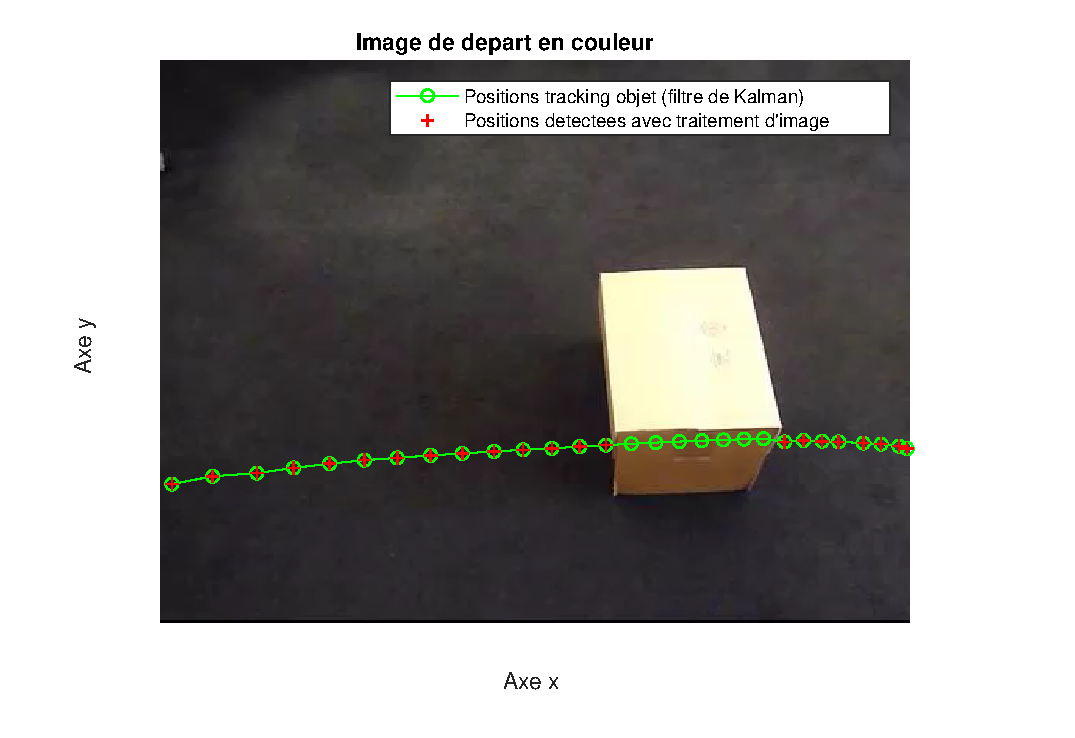
\includegraphics[width=20cm]{Images/Resultats/ImageDeDepartEnCourleur}}
\label{1}
\end{figure}

Sur la figure \ref{1}, les corrections des positions détectées semblent cohérentes. On remarque également que les prédictions des positions de la balle lorsqu'elle n'est pas détectée sont cohérentes.

\begin{figure}[H]
\caption{Positions successives de la balle}
\centerline{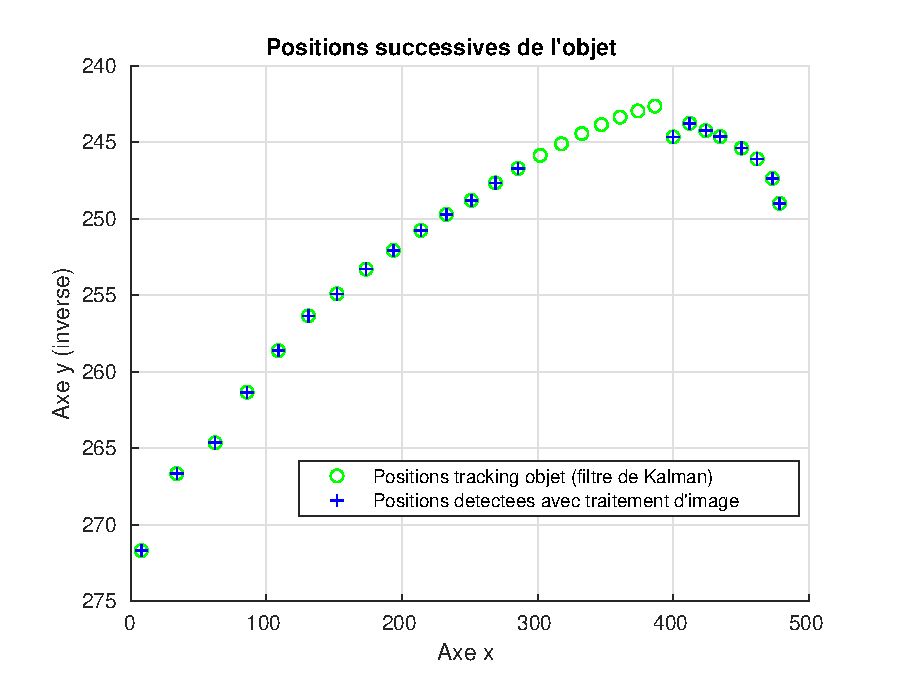
\includegraphics[width=20cm]{Images/Resultats/PositionsSuccessivesDeLObjet}}
\label{2}
\end{figure}

Sur la figure \ref{2}, on peut oberserver avec plus de détail les positions de la balle. On remarque que la prédiction des positions de la balle lorsqu'elle n'est pas détectée s'éloigne de sa vraie position. En effet, au bout de la septième prédiction, on voit que ce point est un peu éloigné de la position détectée lorsque la balle sort de l'autre côté de la boîte.

\subsection{Résultats avec $ dt = 1/30 \; s $ et ajustements de la vitesse et de l'accélération}

\begin{figure}[H]
\caption{Positions successives de la balle \--- Image 1 de la vidéo}
\centerline{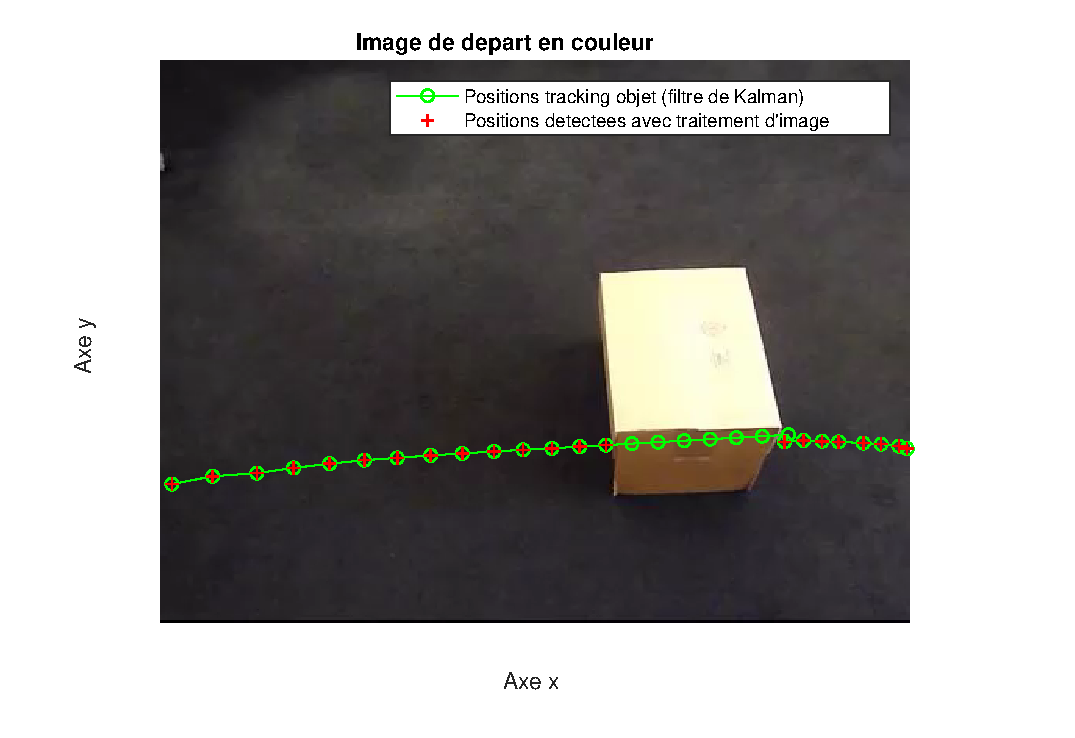
\includegraphics[width=20cm]{Images/Resultats/ImageDeDepartEnCourleur2}}
\label{3}
\end{figure}

Sur la figure \ref{3}, on remarque un problème lorsqu'on prédit la position de la balle quand elle n'est pas détectée. En effet, à la sortie de la boîte, le point prédit est trop loin.

\begin{figure}[H]
\caption{Positions successives de la balle}
\centerline{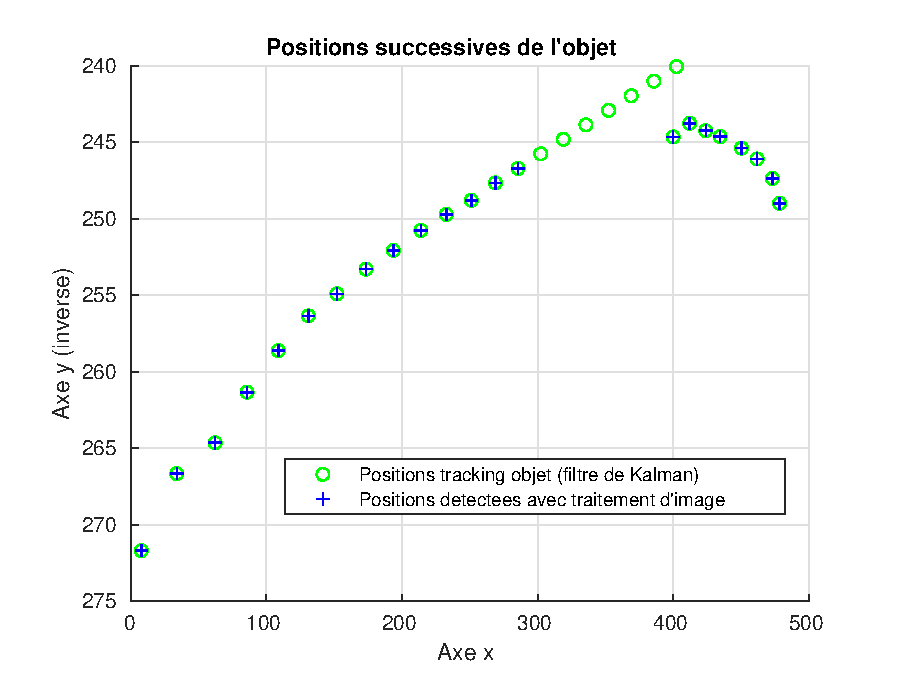
\includegraphics[width=20cm]{Images/Resultats/PositionsSuccessivesDeLObjet2}}
\label{4}
\end{figure}

Sur la figure \ref{4}, on remarque que les prédictions de la position de la balle quand elle n'est pas détectée ne sont pas bonnes. En effet, ces sept points ont une tendance linéaire et le septième point est éloigné du point détecté à la sortie de la boîte.






\newpage
\section{Bibliographie}
\begin{itemize}
\item[•] \textbf{Étude bibliographique sur l'application}
\item[] Applications of Kalman Filtering in Aerospace 1960 to the Present [Historical Perspectives]
\item[] \url{https://ieeexplore.ieee.org/document/5466132/}
\item[] Kalman filter - Applications in Image processing
\item[] \url{https://www.slideshare.net/raviteja1926/kalman-filter-applications-in-image-processing}
\item[] Applications of Kalman Filtering in Aerospace 1960 to the Present
\item[] \url{https://pdfs.semanticscholar.org/b7da/dbff2c53bc30bd910fc0db00e5071a37acfd.pdf}
\item[] Kalman filter
\item[] \url{https://en.wikipedia.org/wiki/Kalman_filter#Example_application}
\item[] Visual Object Tracking using Powell's Direct Set Method and Kalman Filtering
\item[] \url{https://www.youtube.com/watch?v=whwsLjLjEiY}
\item[]
%%
\item[•] \textbf{Explication de l'implémentation}
\item[] MathWorks - Understanding Kalman Filters
\item[] \url{https://fr.mathworks.com/videos/series/understanding-kalman-filters.html}
\item[] MathWorks - configureKalmanFilter (Computer Vision System Toolbox)
\item[] \url{https://fr.mathworks.com/help/vision/ref/configurekalmanfilter.html}
\item[] MathWorks - Using Kalman Filter for Object Tracking
\item[] \url{https://fr.mathworks.com/help/vision/examples/using-kalman-filter-for-object-tracking.html}
\item[] MathWorks - configureKalmanFilter
\item[] \url{https://www.mathworks.com/help/vision/ref/configurekalmanfilter.html#btiaa8o-InitialLocation }
\item[] MathWorks - Vidéos et Webinars - Object Tracking using Kalman Filters
\item[] \url{https://www.mathworks.com/videos/introduction-to-kalman-filters-for-object-tracking-79674.html }
\item[] MathWorks - Tracking Objects: Acquiring and Analyzing Image Sequences in MATLAB
\item[] \url{https://www.mathworks.com/company/newsletters/articles/tracking-objects-acquiring-and-analyzing-image-sequences-in-matlab.html}
\item[] C Code Generation for a MATLAB Kalman Filtering Algorithm
\item[] \url{https://www.mathworks.com/help/coder/examples/c-code-generation-for-a-matlab-kalman-filtering-algorithm.html}
\item[] vision.KalmanFilter class
\item[] \url{https://www.mathworks.com/help/vision/ref/vision.kalmanfilter-class.html }
\item[] Compute Missing data Kalman
\item[] \url{https://stats.stackexchange.com/questions/140990/using-kalman-filters-to-impute-missing-values-in-time-series}

\end{itemize}


\newpage
\section{Annexes}
\subsection{ProjetTSA.m}

\lstset{caption=ProjetTSA.m}
\lstinputlisting{../Code/ProjetTSA.m}

\subsection{trackingObjet.m}

\lstset{caption=trackingObjet.m}
\lstinputlisting{../Code/trackingObjet.m}

\subsection{kalmanFilter.m}

\lstset{caption=kalmanFilter.m}
\lstinputlisting{../Code/kalmanFilter.m}

\subsection{kalmanFilterAjustementsVitesseAcceleration.m}

\lstset{caption=kalmanFilterAjustementsVitesseAcceleration.m}
\lstinputlisting{../Code/kalmanFilterAjustementsVitesseAcceleration.m}

\subsection{kalmanFilterForTracking.m}

\lstset{caption=kalmanFilterForTracking.m}
\lstinputlisting{../Code/kalmanFilterForTracking.m}

\end{document}

